\documentclass[a4paper,12pt]{article}
\usepackage{a4}
\usepackage{epsfig}
\usepackage{listings}
\usepackage{color}
\lstset{language=C++,
        numbers=left,
        numberstyle=\tiny,
        showstringspaces=false,
%        aboveskip=-40pt,
        frame=leftline,
        basicstyle=\ttfamily,
        keywordstyle=\color{red},
        commentstyle=\color{blue},
        breaklines=true,
        xleftmargin=-.075\linewidth,
        linewidth=1.1\linewidth,
        frame=single
        }

\begin{document}

\centerline{\bf\LARGE USBpix and STcontrol with EUDAQ}\ \\[5mm]

Some explanations in this document only concern FE-I4. Most of them are marked,
but as the development is ongoing, there might be some inaccuracies.

This document describes only specialities of the STcontrol EUDAQ integration. 
General information on STcontrol and USBpix can be found at \\
{\tt http://icwiki.physik.uni-bonn.de/twiki/bin/view/Systems/UsbPix}.\\
Instructions are based on USBpixI4 release 5.1 and EUDAQ release 1.3.1. Links to 
the USBpix FE-I3 code are still available, but since this has not been used
with latest EUDAQ and compilers, instructions may not work.

\section{Building STcontrol with EUDAQ integration}

The STcontrol versions with integrated EUDAQ producer can be found in 
svn repositories at the following locations:\\
{\bf FE-I4:} {\tt http://icwiki.physik.uni-bonn.de/svn/USBpixI4/host/}\\
{\bf FE-I3:} {\tt http://icwiki.physik.uni-bonn.de/svn/USBPix/host/}\\
In either case, the {\tt trunk} is fully functional. For FE-I4, as of releases~4.3
 ({\tt tags/release-4.3}) EUDAQ functionality is also included in the 
tagged versions -- see the
release notes for more details. Development branches are out of date 
and should no longer be used.

\subsection{Building EUDAQ}

\subsubsection{Windows with Visual C++ 11.0}

For convenience, USBpix code comes with pre-compiled EUDAQ lib,dll and 
its header files. If a newer version is desired, check out the EUDAQ
code from \\
{\tt http://eudaq.github.io/} \\
% and fix {\tt main/include/eudaq/Platform.hh} if still needed (might 
% be OK in newer versions) after the {\tt \#ifdef WIN32} statement as follows:
% \begin{lstlisting}
% #ifdef WIN32
% #ifdef IN_STCONTROL
% #define DLLEXPORT  __declspec( dllimport ) 
% #else
% #define DLLEXPORT  __declspec( dllexport ) 
% #endif

% #else

% #define DLLEXPORT  

% #endif
% \end{lstlisting}

In order to build the code, follow the EUDAQ instructions using {\tt cmake}.
%Most likely you will need to place pthread pre-built lib and dll files in
%{\tt main/external} --  you will find them in the USBpix package. 
Make sure to build EUDAQ with the same VS version as USBpix!
After having completed the EUDAQ build, copy files from EUDAQ's 
{\tt build/main/lib/Release} or {\tt build/main/lib/Debug} directory (depending 
on tyhe build type you chose) as follows:
\begin{itemize}
\item {\tt EUDAQ.dll} to USBpix's {\tt bin} directory
\item {\tt EUDAQ.lib} to USBpix's {\tt lib} directory
\item the entire content of {\tt include/eudaq} to 
    USBpix's {\tt eudaq/main/include/eudaq} directory
\end{itemize}

\subsubsection{Linux with gcc/g++}\label{sec:eudaq_linux}

Follow the instructions on {\tt http://eudaq.github.io/}
to install EUDAQ.
Afterwards set the environment variable {\tt EUDAQ} to the parent folder 
of your EUDAQ Software, which includes the directory {\tt lib}. 

\subsection{Building STcontrol}

For inclusion of EUDAQ, STcontrol has to be built from scratch, i.e.
all prerequisites as described in the ``insane mode'' of\\
{\tt http://icwiki.physik.uni-bonn.de/twiki/bin/view/Systems/UsbPix\#Installation}
must be followed.

\subsubsection{Windows with Visual C++ 11.0}

Open a command prompt and change location to the main installation
directory of USBpix. Then execute the following commands:
\begin{itemize}
\item {\tt setup -useeudaq yes}
 (to set up environment variables and Makefiles) or if debug printout is needed, call {\bf instead}
\item {\tt setup -useeudaq yes -stcontrol\textunderscore console yes}
\item {\tt nmake} (to compile the code and build the applications)
\end{itemize}
Afterwards you will find an executable called STcontrol\textunderscore eudaq.exe in the bin
directory of the USBpix main directory.

\subsubsection{Linux with gcc/g++}

Linux is fully supported for SLC6 and likely to build on newer distributions such as Fedora 18 and higher. 
Note that libusb-1.0 must be installed, see \\
{\tt http://icwiki.physik.uni-bonn.de/twiki/bin/view/Systems/UsbPix\#Using\textunderscore libusb}.

To build the applications, open a shell (only bash or similar are supported), 
initialise EUDAQ environment (see section~\ref{sec:eudaq_linux}) and
execute:
\begin{itemize}
\item {\tt source setup.sh} 
(to set up environment variables and Makefiles -- presence of EUDAQ should be auto-detected)
\item {\tt make} (to compile the code and build the applications)
\end{itemize}
Afterwards you will find an executable called STcontrol\textunderscore eudaq in the bin
directory of the USBpix main directory.

\section{Starting STcontrol with EUDAQ}

Before starting STcontrol make sure that the EUDAQ Run Control is running and all
USBpix boards are connected and switched on.
Initialise the environment with the setup-scripts as describved for the first step
of building STcontrol in the previous section. STcontrol\textunderscore eudaq(.exe)
offers the following command line parameters:
\begin{itemize}
\item[\bf -r] Run Control IP Connects to a EUDAQ Run Control at the given IP or hostname
directly after start up.
\item[\bf -pid] ProducerID (so far FE-I4 only!). Sets the id of the producer. 
If ProducerID is 0 (default)
the producer will be named {\tt USBpixI4}, otherwise it will be named 
{\tt USBpixI4-\it ProducerID}. This option is only needed to distinguish between multiple USBpix
producers connected to one EUDAQ Run Control. The according configuration
section in the EUDAQ configuration file has to be named like the producer 
({\tt [Producer.USBpixI4]} or {\tt [Producer.USBpixI4-\it ProducerID\tt ]}). 
To distinguish between the sensors connected to the different producers, the parameter 
{\tt first\textunderscore sensor\textunderscore id} in the
EUDAQ configuration file should be used.
\end{itemize}

\section{Configuration of USBpix producer}

\subsection{USBpix settings in the EUDAQ configuration file}

General remarks:
\begin{itemize}
\item Parameters are case sensitive, boolean values (yes/no) and 
trigger\textunderscore replication values not.
\item A default for per board parameters ({\tt parameter[boardid]}) can be set with {\tt parameter[*]}.
{\tt parameter[boardid]} overwrites {\tt parameter[*]}.
\end{itemize}
List of parameters:
\begin{center}
\begin{tabular}{rp{9cm}}
{\bf lvl1\textunderscore delay} & Sets the number of clock cycles between a received trigger and the trigger
send to the FE.\\
{\bf rawdata\textunderscore path} & Path where the raw data in USBpix format is stored. If rawdata\textunderscore path
is not set or empty, no raw data will be stored by STcontrol. This option is
independent from the data storage of EUDAQ.\\
{\bf histogram\textunderscore filename} & Filename for root database to store histograms. If histogram\textunderscore filename
is not set or empty, no local histograms will be stored. Writing of histograms will
slow down the readout.\\
{\bf first\textunderscore sensor\textunderscore id} & Sets the id of the first sensor (order as set in boards parameter) for
LCIO export. Additionally to this value, 10 is added for FE-I3 and 20 for FE-I4.
(Default: 0)\\
{\bf SRAM\textunderscore READOUT\textunderscore AT} & Sets the filling level of the SRAM in percent at which the
SRAM will be read. If this parameter is not set SRAM will be read when it is full.
This parameter is used to ensure synchronous readout of all connected USBpix
boards. The less often the SRAM is read, the shorter the time when USBpix is
busy. If this parameter is chosen too big the large amount of data to be buffered
by EUDAQ data collector and USBpix producer can slow down or even stop the
system.\\
{\bf SkipConfiguration} & If set to ``Yes'' nothing will be done when calling ``Config'' from EUDAQ
Run Control. Configuration has to be done manually in STcontrol.\\
\end{tabular}
\begin{tabular}{rp{9cm}}
{\bf config\textunderscore file} & Filename of the file containing the configuration to be loaded. This can
be either a configuration file for a single board or a multi board configuration
file. If this parameter is set and UseSingleBoardConfig is not set, it has a higher
priority than config\textunderscore file[boardid]. If config\textunderscore file is not set UseSingleBoardConfigs
is automatically set to ``Yes''.\\
{\bf UseSingleBoardConfigs} & If set to ``Yes'' the config\textunderscore file parameter will be neglected and
a multi board configuration will be created from the specified single board configuration
files.\\
{\bf config\textunderscore file[boardid]} & Specifies the config file to be loaded for USBpix board with ID
boardid. The ID has to be activated in the boards parameter. Only available if
UseSingleBoardConfigs is set to ``Yes''.\\
{\bf config\textunderscore module[boardid]} & Name of the module for which the configuration for board
boardid shall be loaded. If config\textunderscore module[boardid] is not set the first module in the
specified configuration file will be used. Only available if UseSingleBoardConfigs
is set to ``Yes''.\\
{\bf boards} & Comma separated list of boards that shall be included in the multi board config
to be created. For every board listed a single board config file has to be specified
in config\textunderscore file[boardid]. Only available if UseSingleBoardConfigs is set to ``Yes''.
fpga\textunderscore firmware Filename of the FPGA firmware to be used. Only available if UseSingleBoardConfigs
is set to ``Yes''.\\
{\bf fpga\textunderscore firmware} & Filename of the FPGA firmware. If fpga\textunderscore firmware is not set or
empty, the default value of the controller class will be used which most likely does not match the paths on your system.
Only available if UseSingleBoardConfigs is set to ``Yes''.\\
{\bf uc\textunderscore firmware} & Filename of the microcontroller firmware. If uc\textunderscore firmware is not set or
empty no new firmware will be loaded into the microcontroller. Only available if
UseSingleBoardConfigs is set to ``Yes''.\\
{\bf adapterCardFlavour} & Flavour of the adapter card connected to the MultiIO board (0: single-chip adapter card SCA, 
1: burn-in card BIC). If not set, a SCA is assumed. Adapter card flavour must match the chip configuration, i.e. must
use BIC in case of DC or QC modules; STcontrol may crash if set wrongly! 
Only available if UseSingleBoardConfigs is set to ``Yes''.\\
\end{tabular}
\begin{tabular}{rp{9cm}}
{\bf trigger\textunderscore replication[boardid]} & Sets the trigger replication (forwarding triggers via a flat
band cable) mode of board with id boardid. Possible values: Master, Slave, Off.
Default value:Off.\\
{\bf tlu\textunderscore trigger\textunderscore data\textunderscore delay} & Sets the delay for reading the trigger number from tlu. Default:
10 (FE-I4), 0 (FE-I3).\\
{\bf trigger\textunderscore rate\textunderscore threshold} & Sets the threshold for reading the SRAM depending on the
trigger rate
\end{tabular}
\end{center}

\subsection{Trigger Replication Mode}

The trigger replication mode was designed to save DUT ports on the TLU. Only one
USBpix system is connected to the TLU, all others are connected via a flat ribbon cable.
To forward the trigger the 16 pin Multi-IO connector is used. Only the pins 1 to 4 of
these pins are nedded and only these 4 pins should be connected as some other pins
are fixed to ground or the supply voltage, which should not be connected between the
boards. This can either be done by using a flat ribbon cable with only 4 lines connected
on standard 16 pin connectors or by using a standard cable and cur 12 of the 16 lines.
Two connected boards are shown in figure~\ref{fig:trgrep}.

If the board connected to TLU has the ID 1 and the other one has the ID 2 the following
lines have to be added to {\tt [Producer.USBpixI4]} section in the EUDAQ configuration file:\\
{\tt trigger\textunderscore replication[1]=Master} \\
{\tt trigger\textunderscore replication[2]=Slave}

\begin{figure}[t]
\centerline{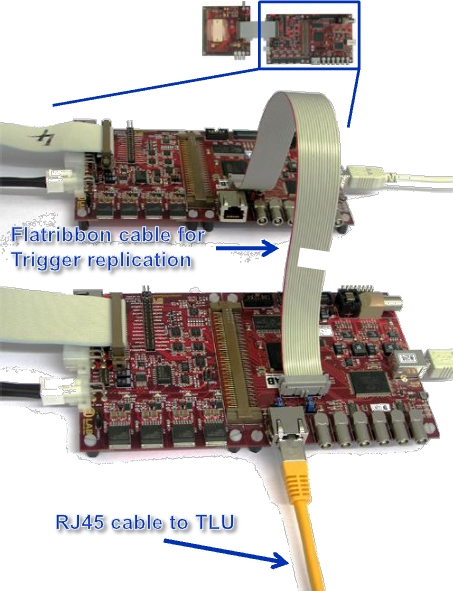
\includegraphics[width=.6\textwidth]{trigger_repl.jpg}}
 \caption{Two USBpix boards connected for trigger replication.\label{fig:trgrep}}
\end{figure}

\subsection{Optimization of tlu\textunderscore trigger\textunderscore data\textunderscore 
delay parameter (FE-I4)}

The default value of {\tt tlu\textunderscore trigger\textunderscore data\textunderscore delay}
is 10. As measurements have shown this
is suitable for RJ45 cables connecting USBpix and a TLU up to 10 meters.

The mean value for a given cable length l can be calculated via 
\[ {\tt tlu\_ trigger\_ data\_ delay}= 0.4\cdot \frac{l}{\rm m}+8.4\, .\]
The communication will work in a parameter range $\pm 3$ 
around this value.
As this value is also strongly dependent on the working speed of the TLU, it might
be necessary to adjust this parameter when using another TLU. Finding the right value
can only be done by trial and error.

\subsection{Example configuration file}\label{sec:exacfg}

The following EUDAQ configuration file serves for a test with two USBpix boards with
fake triggers generated by the TLU.
The configuration for the USBpix producer for FE-I4 is done in the section 
{\tt [Producer.USBpixI4]}. For operation with FE-I3 all available parameters are the same, but a
section called {\tt [Producer.USBpix]} has to be used. When calling {\it Config} from EUDAQ
Run Control USBpix producer will create a new multi board configuration for USBpix
boards with the IDs 38 and 127 from the specified single board configuration files. No raw
data will be stored by STcontrol as {\tt rawdata\textunderscore path} is set empty. 
{\tt SRAM\textunderscore READOUT\textunderscore AT}
is set to 30, which turned out to be a good choice in many tests. For board 38 the trigger
replication mode is set to master. It has to be connected to TLU via the RJ45 port and
to all other boards via a flat band cable. All other boards are configures as replication
slave, as the default parameter {\tt trigger\textunderscore replication[*]} is used.
In section {\tt [Producer.TLU]} the TLU is configured to send fake triggers to two boards
connected to the ports 0 and 1 with a frequency of 1 kHz. For proper operation with
USBpix the parameter {\tt EnableDUTVeto} has to be set for all USBpix boards. Encoding
of this parameter and other parameters in this configuration file can be found in the
EUDAQ Software User Manual.

\begin{lstlisting}
[RunControl]
RunSizeLimit = 100000000
NoTrigWarnTime = 10

[DataCollector]

[LogCollector]
SaveLevel = ALL
PrintLevel = WARN

[Producer.TLU]
AndMask = 0
OrMask = 0
VetoMask = 0
TriggerInterval = 1
EnableDUTVeto = 3
DutMask = 3
BitFile = ../tlu/TLU2_Toplevel−65_40MHz.bit

[Producer.USBpixI4]
SkipConfiguration=no
UseSingleBoardConfig=Yes
boards=38,127
config_file[38]= config\std_with_DCS.cfg.root
config_file[127]= config\std_with_DCS.cfg.root
fpga_firmware=C:\icwiki_svn\USBPixI4\host\tags\rerlease-4.3\config\usbpixi4.bit
rawdata_path=
SRAM_READOUT_AT=30
trigger_replication[38] = Master
trigger_replication[*] = Slave

\end{lstlisting}

\section{Known Problems}

\begin{itemize}
\item USBpix won't work with USB hubs.
\item Sometimes powering via USB is unstable, thus better use external powering.
\item If trigger sending stops after first SRAM readout, the parameter {\tt EnableDUTVeto}
isn't set correctly for the TLU, see section~\ref{sec:exacfg}.
\item Sometimes USBpix stucks sending data to the Data Collector. This can have
several reasons, but the symptom is always the same: The number of Particles
and Trigger in the EUDAQ Run Control is continously increasing, but the Events
build don’t cange and are more than 50000 lower than Triggers. As USBpix send
events more frequently at the beginning of a run one can also see this promblem if
Events Build stays 0, but Trigger is $> 10000$. In this case stop the run and restart
STcontrol. If the problem appears again afterward one also needs to re power the
USBpix system and restart STcontrol.
\item If the hostname of the Run Control PC cannot be resolved via DNS and one tries
to connect by using the IP Address, the producer will conenct to Run Control,
but fail to connect to Data and Log Collector. Thus configuring will work, but
no events will be build while scanning. To avoid this add an entry with hostname
and IP Adress to \\
{\tt C:\textbackslash Windows\textbackslash System32\textbackslash drivers\textbackslash etc\textbackslash hosts}.
\end{itemize}

\end{document}
